\begin{section}{Numerical integration of the equations of motion: the case of the Vortex}\label{ann:num}
  We assume that the field equations for the two degrees of freedom
  $A$ and $F$ are known, and given by
  \begin{align}
    \begin{aligned}
      &-\frac{\mathrm d}{\mathrm d r}\left[r\frac{\mathrm d F}{\mathrm dr}\right]+\lambda v^2 r (F^2-1)F+ \frac{F}{r}(A-1)^2 = 0,\\
      &-\frac{\mathrm d}{\mathrm d r}\left[\frac{1}{r}\frac{\mathrm d A}{\mathrm d r}\right] - 2e^2v^2\frac{F^2(1-A)}{r} = 0
    \end{aligned}\label{eq:fequs}
  \end{align}
  with the following asymptotic behaviour:
  \begin{align}
    &F(r) \to 1,\qquad A(r) \to 1,\qquad \text{as }r\to \infty,\\
    &F(r) \to 0,\qquad A(r) \to 0,\qquad \text{as }r\to 0.
  \end{align}
  
  We are looking for a numerical scheme which converge to a solution
  of (\ref{eq:fequs}) satisfiying these boundary conditions. Let's
  define for convenience the two auxiliary functions:
  \begin{align}
    M(r,x,y) = \alpha r^2(y^2-1)y,\\
    N(r,x,y) = \beta ry^2(1-x)
  \end{align}
  such that the system to solve reads:
  \begin{align}
    \left\{\begin{aligned}
      r^2F''+rF'-M(r,A,F) = 0,\\
      rA''-A'+N(r,A,F) = 0.
    \end{aligned}\right.\label{eq:nonlinsyst}
  \end{align}
  The boundary condition at infinity is hard to implement, so in a
  first approximation, we choose a maximal radius $R$ where both
  function $A$ and $F$ eventually reach 1. We hope that the result of
  the simulation will be a good approximation of the solution if $R$
  is sufficiently large.
  
  We discretize the interval $[0,R]$ into $N$ points uniformly distributed
  \begin{equation}
    r_i = ih,\quad h = \frac{R}{N+1} \quad\Longrightarrow\quad r_0 = 0,\ r_{N+1} = R,
  \end{equation}
  and we write
  \begin{equation}
    a_i = A(r_i),\quad f_i = F(r_i).
  \end{equation}
  The non-linear system (\ref{eq:nonlinsyst}) gives rise to the following
  finite differences scheme:
  \begin{align}
    \frac{r_i^2}{h^2}\left(f_{i+1}-2f_i+f_{i-1}\right)+\frac{r_i}{2h}\left(f_{i+1}-f_{i-1}\right) - M(r_i, a_i, f_i) = 0,\\
    \frac{r_i}{h^2}\left(a_{i+1}-2a_i+a_{i-1}\right)-\frac{1}{2h}\left(a_{i+1}-a_{i-1}\right) + N(r_i, a_i, f_i) = 0
  \end{align}
  $\forall\ i = 1,\dots,N$ with the boundary conditions:
  \begin{equation}
    a_0 = f_0 = 0,\quad a_{N+1} = f_{N+1} = 1.
  \end{equation}
%  \begin{figure}[h!]
%    % GNUPLOT: LaTeX picture with Postscript
\begingroup
  \makeatletter
  \providecommand\color[2][]{%
    \GenericError{(gnuplot) \space\space\space\@spaces}{%
      Package color not loaded in conjunction with
      terminal option `colourtext'%
    }{See the gnuplot documentation for explanation.%
    }{Either use 'blacktext' in gnuplot or load the package
      color.sty in LaTeX.}%
    \renewcommand\color[2][]{}%
  }%
  \providecommand\includegraphics[2][]{%
    \GenericError{(gnuplot) \space\space\space\@spaces}{%
      Package graphicx or graphics not loaded%
    }{See the gnuplot documentation for explanation.%
    }{The gnuplot epslatex terminal needs graphicx.sty or graphics.sty.}%
    \renewcommand\includegraphics[2][]{}%
  }%
  \providecommand\rotatebox[2]{#2}%
  \@ifundefined{ifGPcolor}{%
    \newif\ifGPcolor
    \GPcolortrue
  }{}%
  \@ifundefined{ifGPblacktext}{%
    \newif\ifGPblacktext
    \GPblacktexttrue
  }{}%
  % define a \g@addto@macro without @ in the name:
  \let\gplgaddtomacro\g@addto@macro
  % define empty templates for all commands taking text:
  \gdef\gplbacktext{}%
  \gdef\gplfronttext{}%
  \makeatother
  \ifGPblacktext
    % no textcolor at all
    \def\colorrgb#1{}%
    \def\colorgray#1{}%
  \else
    % gray or color?
    \ifGPcolor
      \def\colorrgb#1{\color[rgb]{#1}}%
      \def\colorgray#1{\color[gray]{#1}}%
      \expandafter\def\csname LTw\endcsname{\color{white}}%
      \expandafter\def\csname LTb\endcsname{\color{black}}%
      \expandafter\def\csname LTa\endcsname{\color{black}}%
      \expandafter\def\csname LT0\endcsname{\color[rgb]{1,0,0}}%
      \expandafter\def\csname LT1\endcsname{\color[rgb]{0,1,0}}%
      \expandafter\def\csname LT2\endcsname{\color[rgb]{0,0,1}}%
      \expandafter\def\csname LT3\endcsname{\color[rgb]{1,0,1}}%
      \expandafter\def\csname LT4\endcsname{\color[rgb]{0,1,1}}%
      \expandafter\def\csname LT5\endcsname{\color[rgb]{1,1,0}}%
      \expandafter\def\csname LT6\endcsname{\color[rgb]{0,0,0}}%
      \expandafter\def\csname LT7\endcsname{\color[rgb]{1,0.3,0}}%
      \expandafter\def\csname LT8\endcsname{\color[rgb]{0.5,0.5,0.5}}%
    \else
      % gray
      \def\colorrgb#1{\color{black}}%
      \def\colorgray#1{\color[gray]{#1}}%
      \expandafter\def\csname LTw\endcsname{\color{white}}%
      \expandafter\def\csname LTb\endcsname{\color{black}}%
      \expandafter\def\csname LTa\endcsname{\color{black}}%
      \expandafter\def\csname LT0\endcsname{\color{black}}%
      \expandafter\def\csname LT1\endcsname{\color{black}}%
      \expandafter\def\csname LT2\endcsname{\color{black}}%
      \expandafter\def\csname LT3\endcsname{\color{black}}%
      \expandafter\def\csname LT4\endcsname{\color{black}}%
      \expandafter\def\csname LT5\endcsname{\color{black}}%
      \expandafter\def\csname LT6\endcsname{\color{black}}%
      \expandafter\def\csname LT7\endcsname{\color{black}}%
      \expandafter\def\csname LT8\endcsname{\color{black}}%
    \fi
  \fi
  \setlength{\unitlength}{0.0500bp}%
  \begin{picture}(6236.00,2834.00)%
    \gplgaddtomacro\gplbacktext{%
      \csname LTb\endcsname%
      \put(946,704){\makebox(0,0)[r]{\strut{} 0}}%
      \put(946,1077){\makebox(0,0)[r]{\strut{} 0.2}}%
      \put(946,1450){\makebox(0,0)[r]{\strut{} 0.4}}%
      \put(946,1823){\makebox(0,0)[r]{\strut{} 0.6}}%
      \put(946,2196){\makebox(0,0)[r]{\strut{} 0.8}}%
      \put(946,2569){\makebox(0,0)[r]{\strut{} 1}}%
      \put(1078,484){\makebox(0,0){\strut{} 0}}%
      \put(1758,484){\makebox(0,0){\strut{} 1}}%
      \put(2438,484){\makebox(0,0){\strut{} 2}}%
      \put(3118,484){\makebox(0,0){\strut{} 3}}%
      \put(3799,484){\makebox(0,0){\strut{} 4}}%
      \put(4479,484){\makebox(0,0){\strut{} 5}}%
      \put(5159,484){\makebox(0,0){\strut{} 6}}%
      \put(5839,484){\makebox(0,0){\strut{} 7}}%
      \put(176,1636){\rotatebox{-270}{\makebox(0,0){\strut{}$A(r)$, $F(r)$}}}%
      \put(3458,154){\makebox(0,0){\strut{}Radius $r$}}%
    }%
    \gplgaddtomacro\gplfronttext{%
      \csname LTb\endcsname%
      \put(4852,2396){\makebox(0,0)[r]{\strut{}$A(r)$}}%
      \csname LTb\endcsname%
      \put(4852,2176){\makebox(0,0)[r]{\strut{}$F(r)$}}%
    }%
    \gplbacktext
    \put(0,0){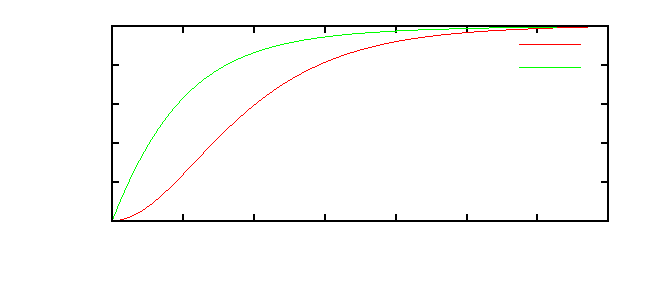
\includegraphics{a_and_f_funcs_vortex}}%
    \gplfronttext
  \end{picture}%
\endgroup

%    \caption{\em Numerical integration of the non-linear system of
%      equation for the vortex. We have chosen $R = 7$, $N = 400$,
%      $\alpha = \beta = 1$. We note that obviously, for $r\to 0$, we
%      have $f(r)\neq O(r^2)$.}
%    \label{fig:a_and_f_funcs}
%  \end{figure}
  In order to solve for the unknown $a_i$, $f_i$, let's write
  \begin{equation}
    x_i =\left\{ 
    \begin{aligned}
      &a_i,\quad\forall i = 1,\dots,N\\
      &f_i,\quad\forall i = N+1,\dots,2N\\
    \end{aligned}\right.
  \end{equation}
  and the numerical scheme becomes
  \begin{equation}
    \vec g(x_1,\dots,x_{2N}) = 
    \begin{bmatrix}
      g_1(x_1, \dots, x_{2N})\\
      \vdots\\
      g_{2N}(x_1, \dots, x_{2N})\\
    \end{bmatrix}
    = 
    \begin{bmatrix}
      0\\
      \vdots\\
      0
    \end{bmatrix}
  \end{equation}
  where
  \begin{align}
    g_1(x) &= \frac{r_1}{h^2}\left(x_2-2x_1\right)-\frac{1}{2h}x_2+N(r_1,x_1,x_{N+1}),\\
    g_N(x) &= \frac{r_N}{h^2}\left(1-2x_N+x_{N-1}\right)-\frac{1}{2h}\left(1-x_{N-1}\right)+N(r_N,x_N,x_{2N}),\\
    g_{N+1}(x)& = \frac{r_1^2}{h^2}\left(x_{N+2}-2x_{N+1}\right)+\frac{r_1}{2h}x_{N+2}-M(r_1,x_1, x_{N+1}),\\
    g_{2N}(x) &= \frac{r_N^2}{h^2}\left(1-2x_{2N}+x_{2N-1}\right)+\frac{r_N}{2h}\left(1-x_{2N-1}\right)-M(r_N,x_N, x_{2N}),
  \end{align}
  \begin{multline}
    g_i(x) = \frac{r_i}{h^2}\left(x_{i+1}-2x_i+x_{i-1}\right)-\frac{1}{2h}\left(x_{i+1}-x_{i-1}\right),\\
    +N(r_i, x_i, x_{N+i}),\quad
    \forall i = 2,\dots,N-1,\\
  \end{multline}
  \begin{multline}
    g_i(x) = \frac{r_{i-N}^2}{h^2}\left(x_{i+1}-2x_i+x_{i-1}\right)-\frac{r_{i-N}}{2h}\left(x_{i+1}-x_{i-1}\right),\\
    +M(r_{i-N}, x_{i-N}, x_i),\quad
    \forall i = N+2,\dots,2N-1.\\    
  \end{multline}
  We then use Newton-Raphson iteration to find the solution for the
  $x_i$'s:
  \begin{equation}
    x^{i+1} = x^i - \frac{\vec g(x)}{J[\vec g]_x}\quad \Longleftrightarrow\quad J[\vec g]_x^{-1}\left(x^{i+1}-x^i\right) = \vec g(x)
  \end{equation}
  where $J[\vec g]_x$ is the Jacobian matrix of $\vec g$ evaluated at
  $x$. The solution is given by $x = \lim_{i\to\infty}x^i$, and the
  convergence is faster if we choose cleverly the initial point $x^0$.
  %The results are shown on Fig. \ref{fig:a_and_f_funcs}.
\end{section}
